\subsection*{Træning} \label{sec:traening}
Brugeren har mulighed for at fortage træninger baseret på forskellige træningsformer og træningstyper. Derudover skal træningen kunne tilpasses individuelt under hver enkelt træningssession, samt tilkolbe yderligere måleenheder for at opnå en mere vejledende og fyldestgørende træning.  
Aktivitetsdiagrammet over træningen fremgår af \autoref{fig:traening}. 

\begin{figure} [H]
\centering
\textbf{Aktivitetsdiagram: Træning}\par\medskip
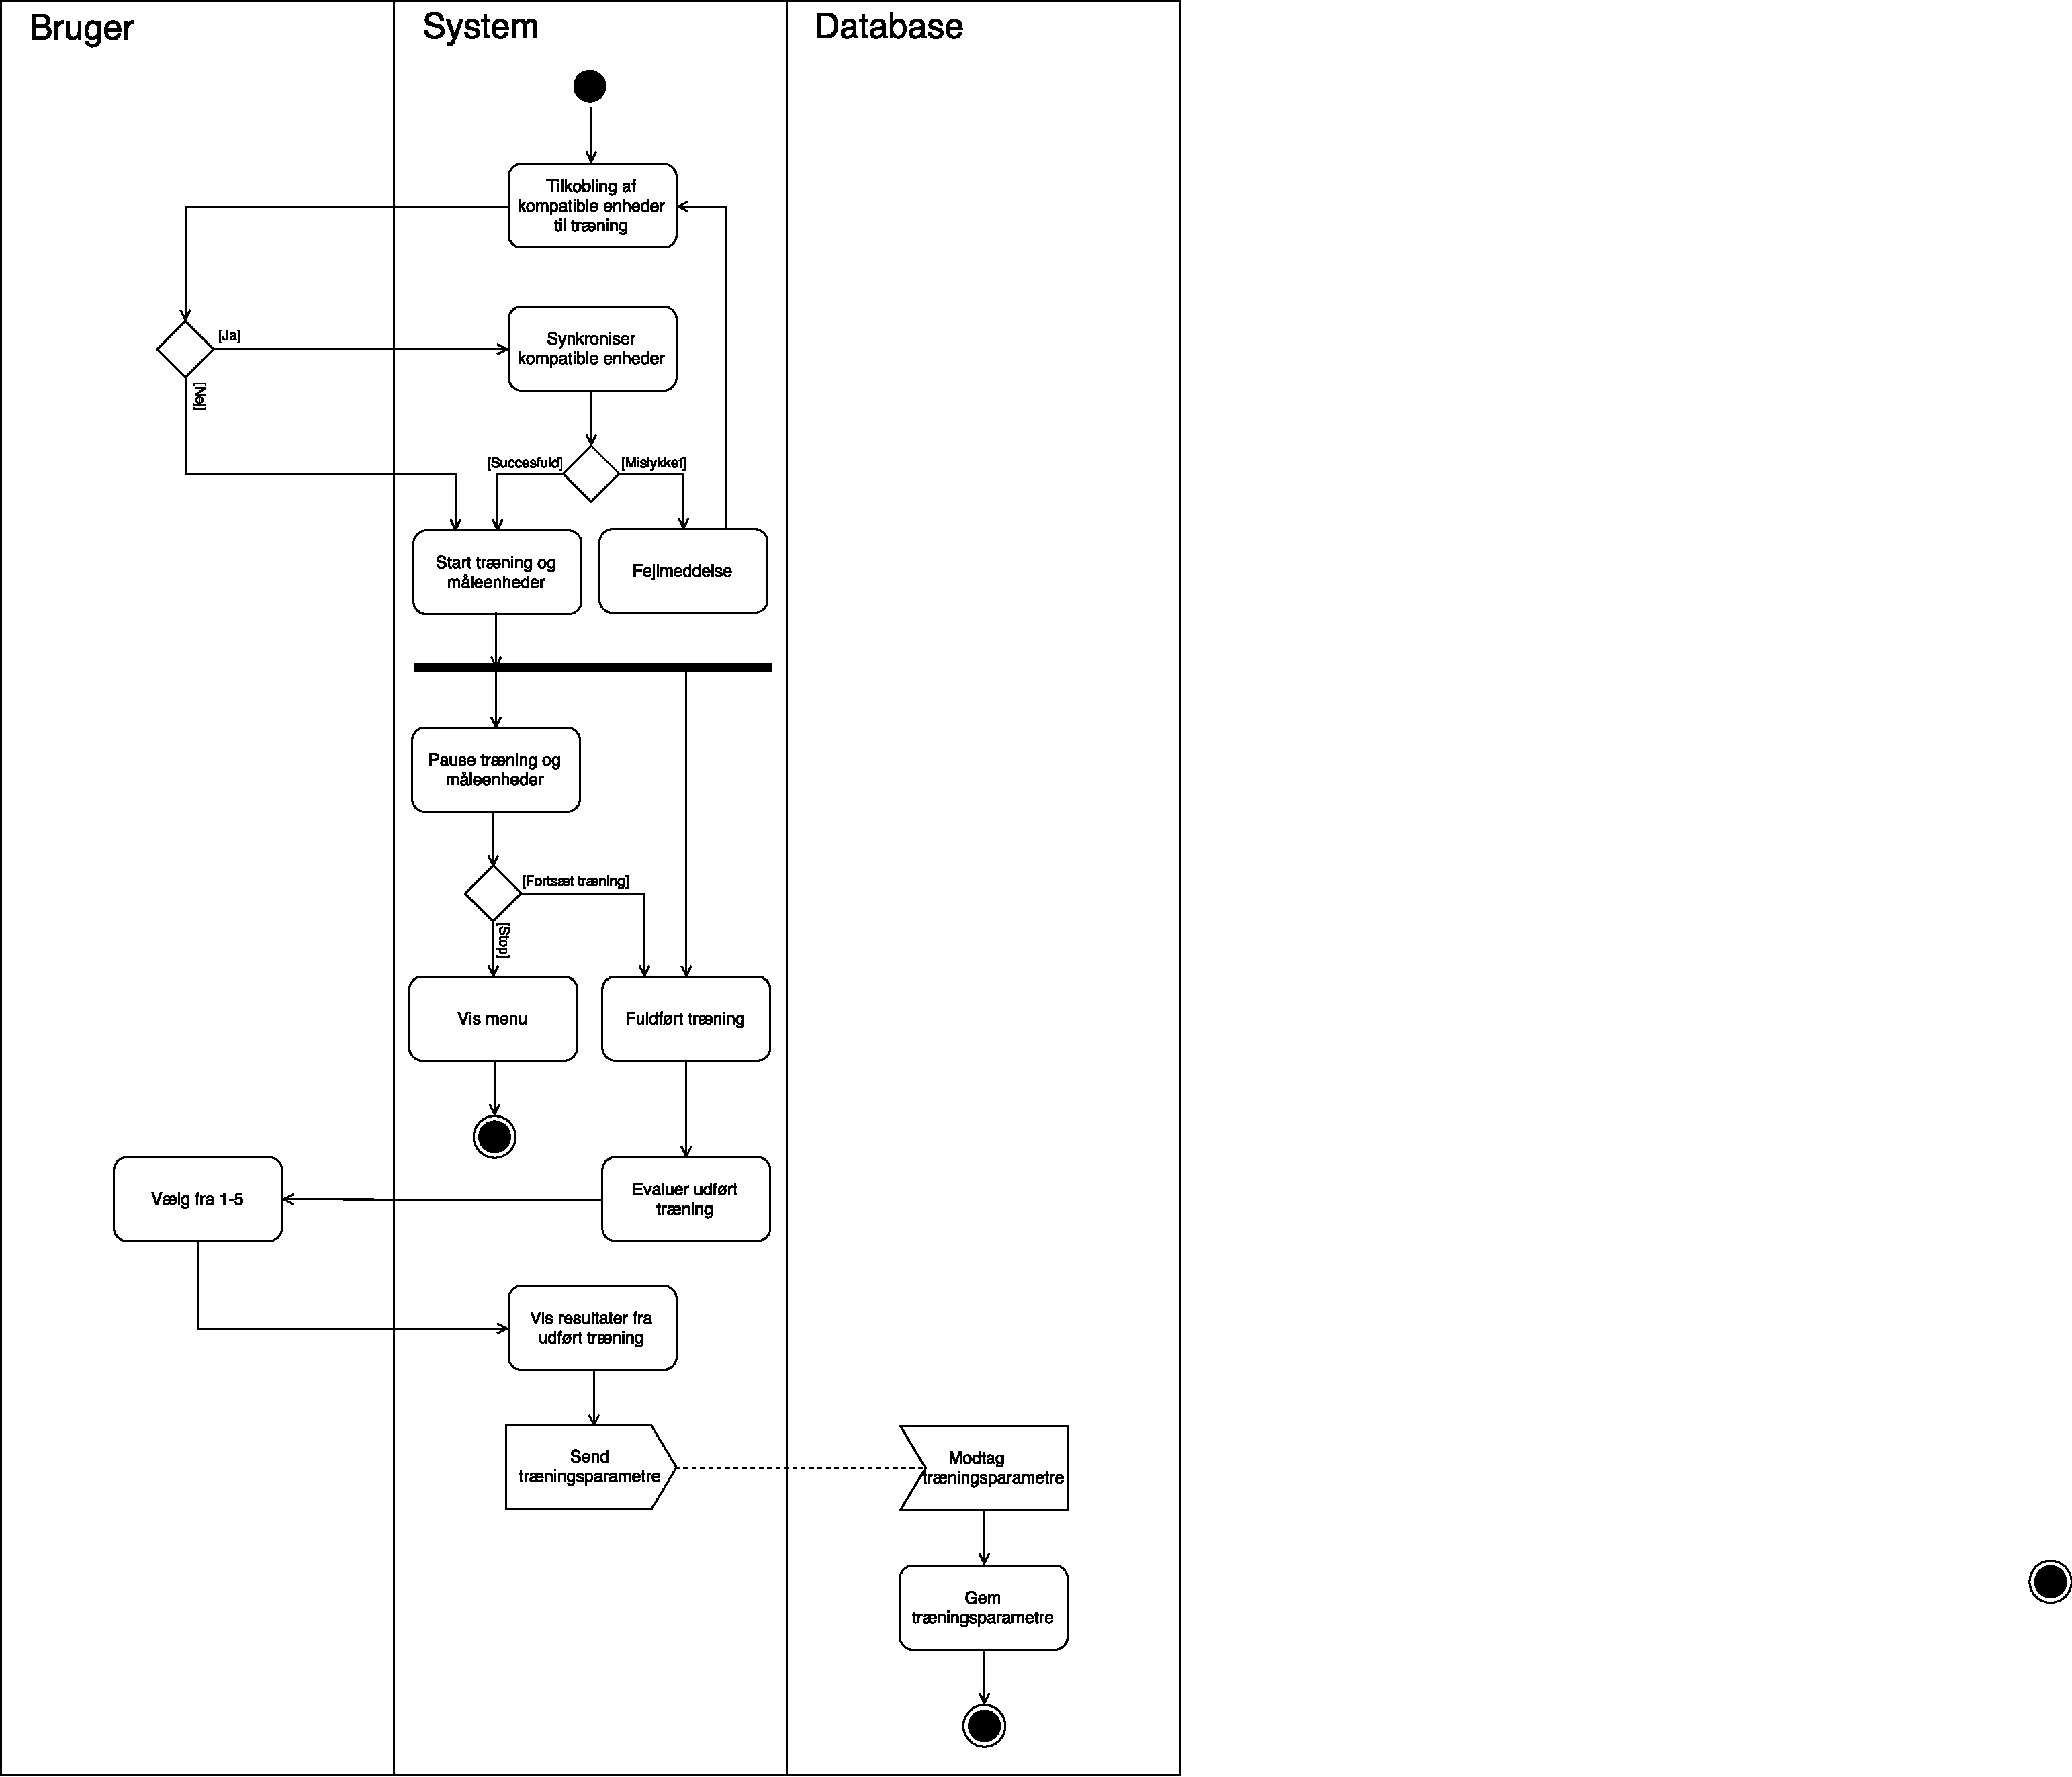
\includegraphics[width=0.8\textwidth]{figures/aktivitetsdiagram/Traening}
\caption{Aktivitetsdiagram over træning.}
\label{fig:traening}
\end{figure}

\noindent
Før selve træningen påbegyndes, skal brugeren angive den ønskede træningsform, herunder konditions-, styrketræning eller vejrtrækningsøvelser. Ud fra den valgte træningsform skal brugeren angive træningstype, eksempelvis kan der i forlængelse af konditionstræning vælges gå, løbe eller cykle. 
Efterfølgende tilpasses træningsniveauet til den enkelte bruger, og er beskrevet af et særskilt aktivitetsdiagram i \autoref{fig:traeningsniveau}.
Systemet vil efterfølgende undersøge om der er kompatible måleenheder til rådighed, og tilkoble dem til træningen før den påbegyndes af brugeren. 
Under træningen vil systemet kontinuert vise træningen og målinger der fortages. Brugeren kan til hver en tid vælge at afslutte træningen, dog skal denne handlingen bekræftes i tilfælde af at brugeren ved fejl angiver at træningen skal stoppes. 
Systemet stopper dermed træningen og afventer en evalueringen som skal angives af brugeren. 
Efter at træningssættet er evalueret sender systemet informationen relateret til træningssessionen til databasen, hvor det gemmes.  

\subsection*{Tilpasning af træningsniveau} \label{sec:traeningsniveau}
Tilpasning af træningsniveau er en funktion der skal varetage træningen for brugeren, ved at anbefale et træningsniveau ud fra brugeres kategorisering, dag til dag variationer og tidligere evalueringer af træninger. Aktivitetsdiagrammet over valg af træningsniveau fremgår af \autoref{fig:traening}.
 
\begin{figure} [H]
\centering
\textbf{Aktivitetsdiagram: Valg af træningsniveau}\par\medskip
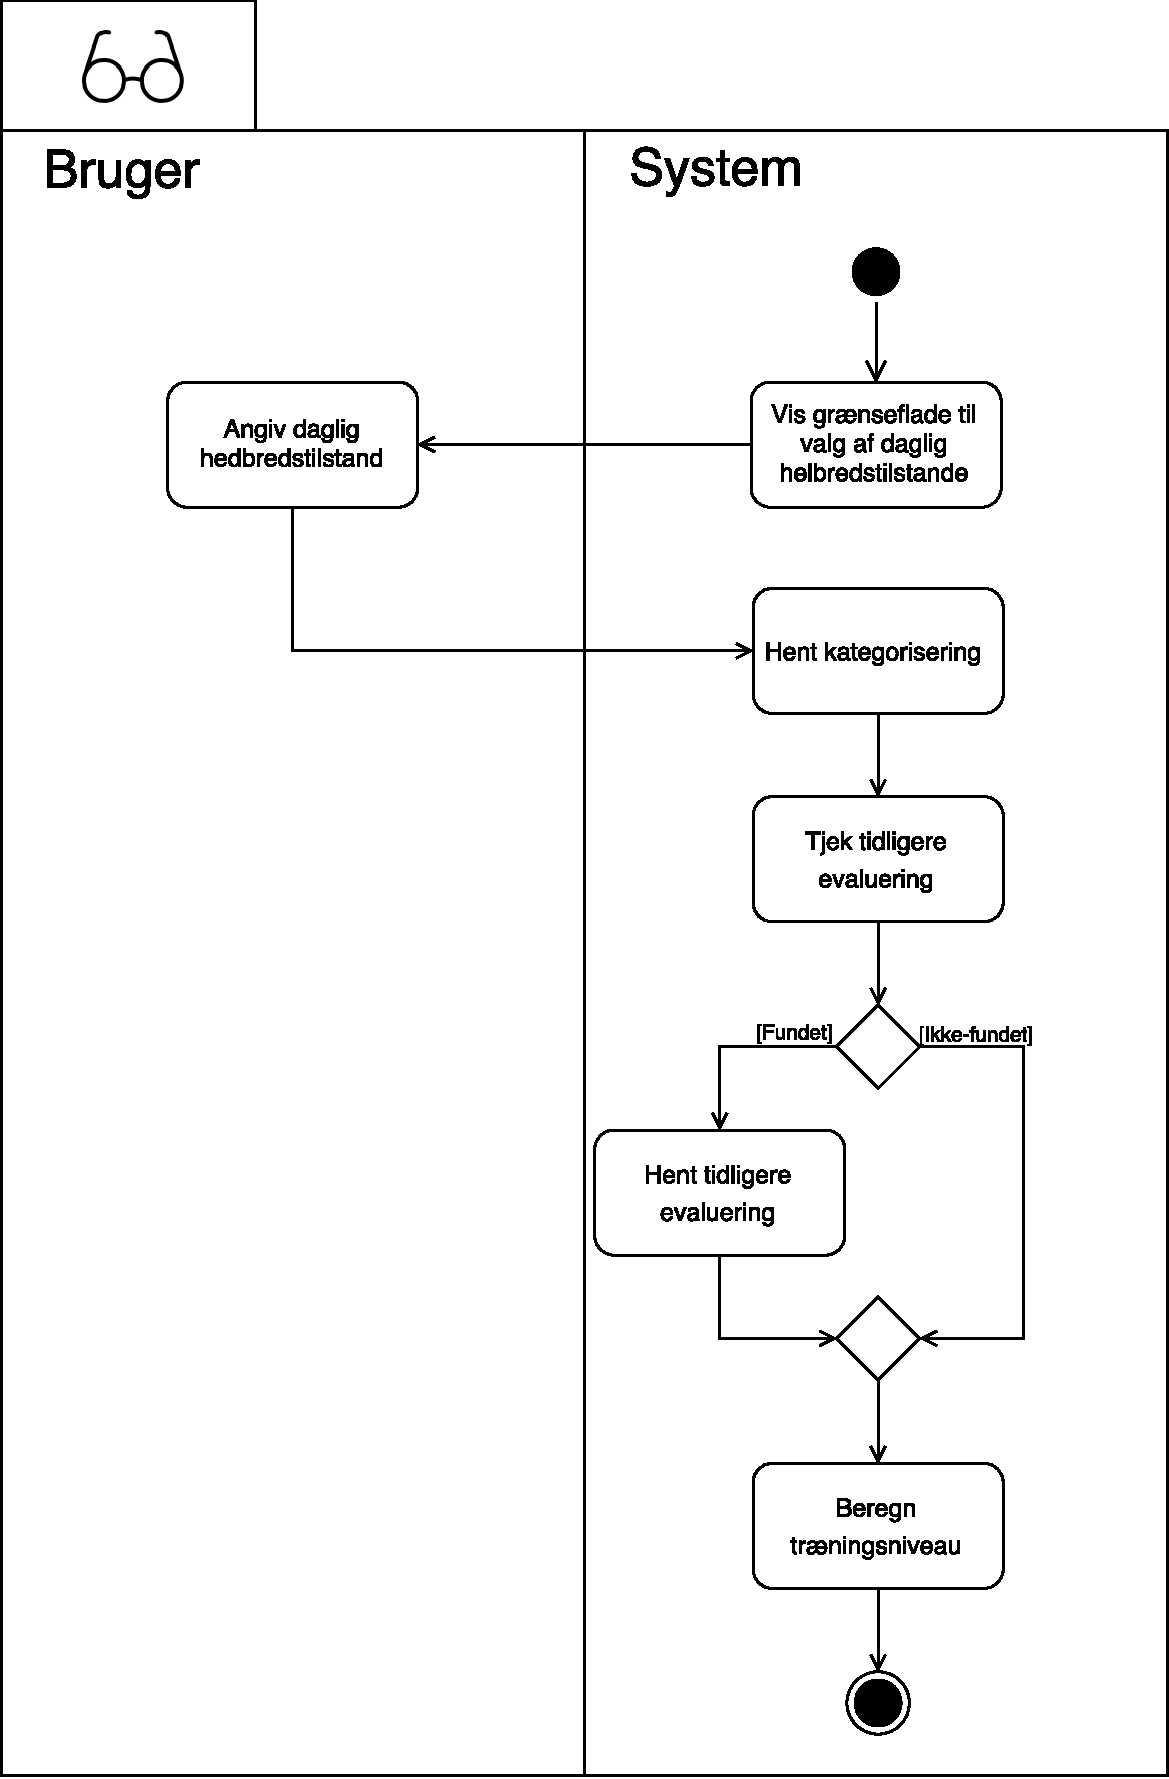
\includegraphics[width=0.8\textwidth]{figures/aktivitetsdiagram/Tilpasningaftraeningsniveau}
\caption{Aktivitetsdiagram over valg af træningsniveau.}
\label{fig:traeningsniveau}
\end{figure}

\noindent
Valg af træningsniveau ses som en aktivitet i aktivitetsdiagrammet for træning i \autoref{fig:traening}. For at systemet kan tilpasse træningsniveauet, vil brugeren skulle angive sin helbredstilstand før den givne træning. Yderligere beregnes træningsniveauet af brugers kategorisering, som blev defineret første gang brugeren loggede ind på app'en, og på tidligere evalueringer, såfremt tidligere evalueringer er fortaget.


Tilpasningen af træningsniveauet kan også visualiseres som en simpel beslutningstabel, der ses af \autoref{tab:beslutningstabel}. Tabellen beskriver hvordan en algoritme, ville regulere i træningsniveauet således det er passende til den enkelte bruger.  

\subsubsection*{Algoritme til tilpasning af træningsniveau}
Algoritmen til valg af træningsniveau er illustreret som en simpel beslutningstabel, der viser, hvilke parameter, som ligger til grund for valg af træningsniveau til den enkelte bruger. Af \autoref{tab:beslutningstabel} ses beslutningstabellen for valg af træningsniveau.

\begin{table}[H]
\centering
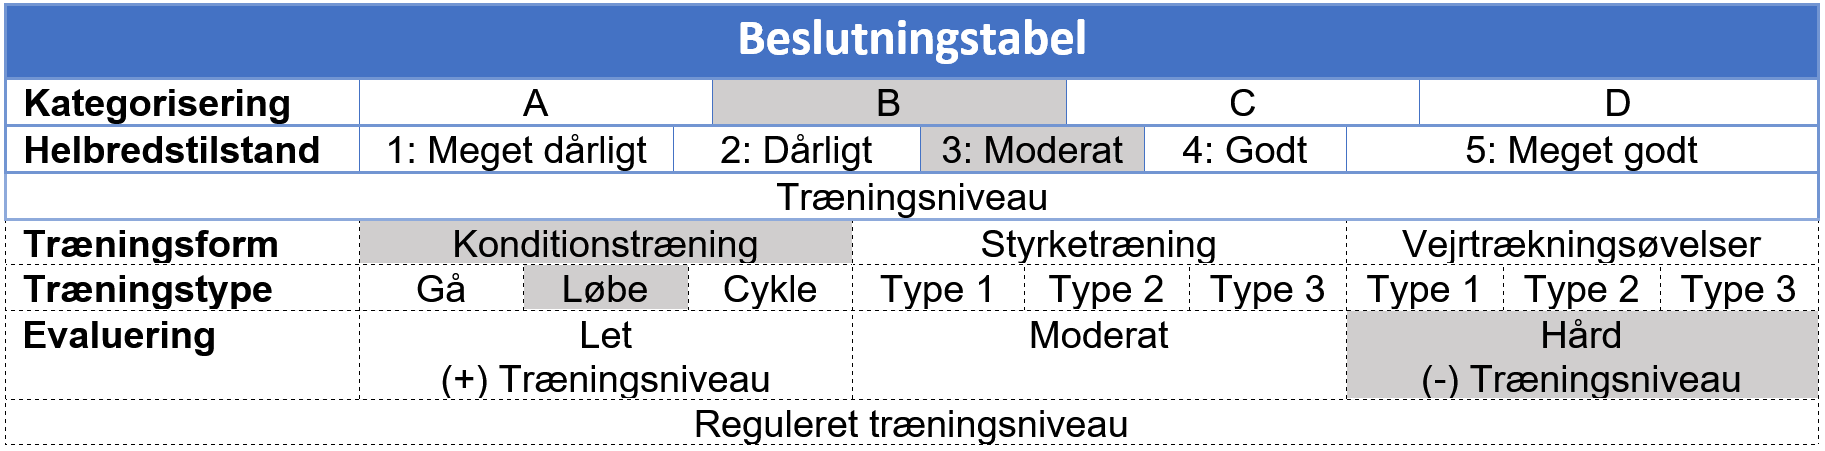
\includegraphics[width=1\textwidth]{figures/aktivitetsdiagram/beslutningstabel}
\caption{Beslutningstabel for træningsniveau. Kategorisering, daglig helbredstilsand samt eventuel evaluering medregnes til at bestemme træningsniveau til den enkelte træning. Af dette eksempel er brugeren kategoriseret B med en helbredstilstand, der er angivet som moderat. Dertil har brugeren valgt løb under konditionstræning. Tidligere har brugeren haft samme daglig helbredstilstand samt træning, og evalueret denne træning som værende hård. Dette muliggøre en regulering af træningsniveauet, hvorfor niveauet i dette tilfælde sænkes.}
\label{tab:beslutningstabel}
\end{table} 

\noindent
Af \autoref{tab:beslutningstabel} fremgår en simpel beslutningstabel for, hvorledes et træningssæt tilpasses den enkelte bruger. Beslutningstabellen tager udgangspunkt i brugerens kategorisering, daglig helbredstilstand samt en eventuel evaluering. Brugeren er i dette tilfælde kategoriseret til B. Helbredstilstanden angives førend en træning påbegyndes, for således at tilpasse niveauet til den pågældende dag. Helbredstilstanden angives efter \textit{1: Meget dårligt}, \textit{2: Dåligt}, \textit{3: Moderat}, \textit{4: Godt} eller \textit{5: Meget godt}, hvortil brugerens helbredstilstand her angives som moderat
Træningsniveauet vurderes dermed ud fra brugerens kategorisering samt helbredstilstand. 
For at have mulighed for at kunne regulere træningssættet yderligere, medregnes den forhenværende evaluering, der er forbundet med samme helbredstilstand, træningsform og type. I dette tilfælde har brugeren før haft samme helbredstilstand, træningsform samt type og dertil evalueret denne træning til værende hård. Algoritmen regulerer hertil træningsniveauet for denne træning ned, for således at give brugeren en bedre træningsoplevelse. 
